%
% $Id: ch02_relatedwork
%
%   *******************************************************************
%   * SEE THE MAIN FILE "AllegThesis.tex" FOR MORE INFORMATION.       *
%   *******************************************************************
\chapter{Related Work}\label{ch:relatedwork}

Intro paragraph here.

\section{Primary Sources}
Though I will not be comparing existing images located in a database, the paper by Lee, Ke, and Isard \cite{Lee:2010} can be useful in method of approach. During their research they utilized a partition min-hash function for discovering near-duplicate images. Partition by hash functions are used to break down a large data set into a number of equal sized segments that can be identified by a generated hash. Instead of looking at the image as a whole as many other algorithms do, it looks at the image as several smaller pieces through the use of the partition hashing function. They claimed that the algorithm is actually faster and more effective than standard min-hash functions which look at the entire image. Since the proposed research I will be performing is highly efficiency sensitive due to its web based structure, I will consider implementing a variant of this method of comparison.

Another article that will be vital to creating an effective and efficient image matching algorithm will be the 2010 paper by Srinivasan. This research was targeted at web-based image matching, which is exactly what I am going to perform. This research claims that traditional near-duplicate detection systems are not applicable for the de-duplication of large-scale web image collections, \cite{Srinivasan:2008} the research performed targeted an image matching system which was scalable, highly efficient, and effective.

In order to perform the effective image matching the authors required, they decided to implement a thumbnail matching based system. This algorithm would generate a 130-bit thumbnail representation of the image and was capable of finding near-duplicate images while operating in $O(1)$ time \cite{Srinivasan:2008}.

\begin{figure}[htbp]
\centering
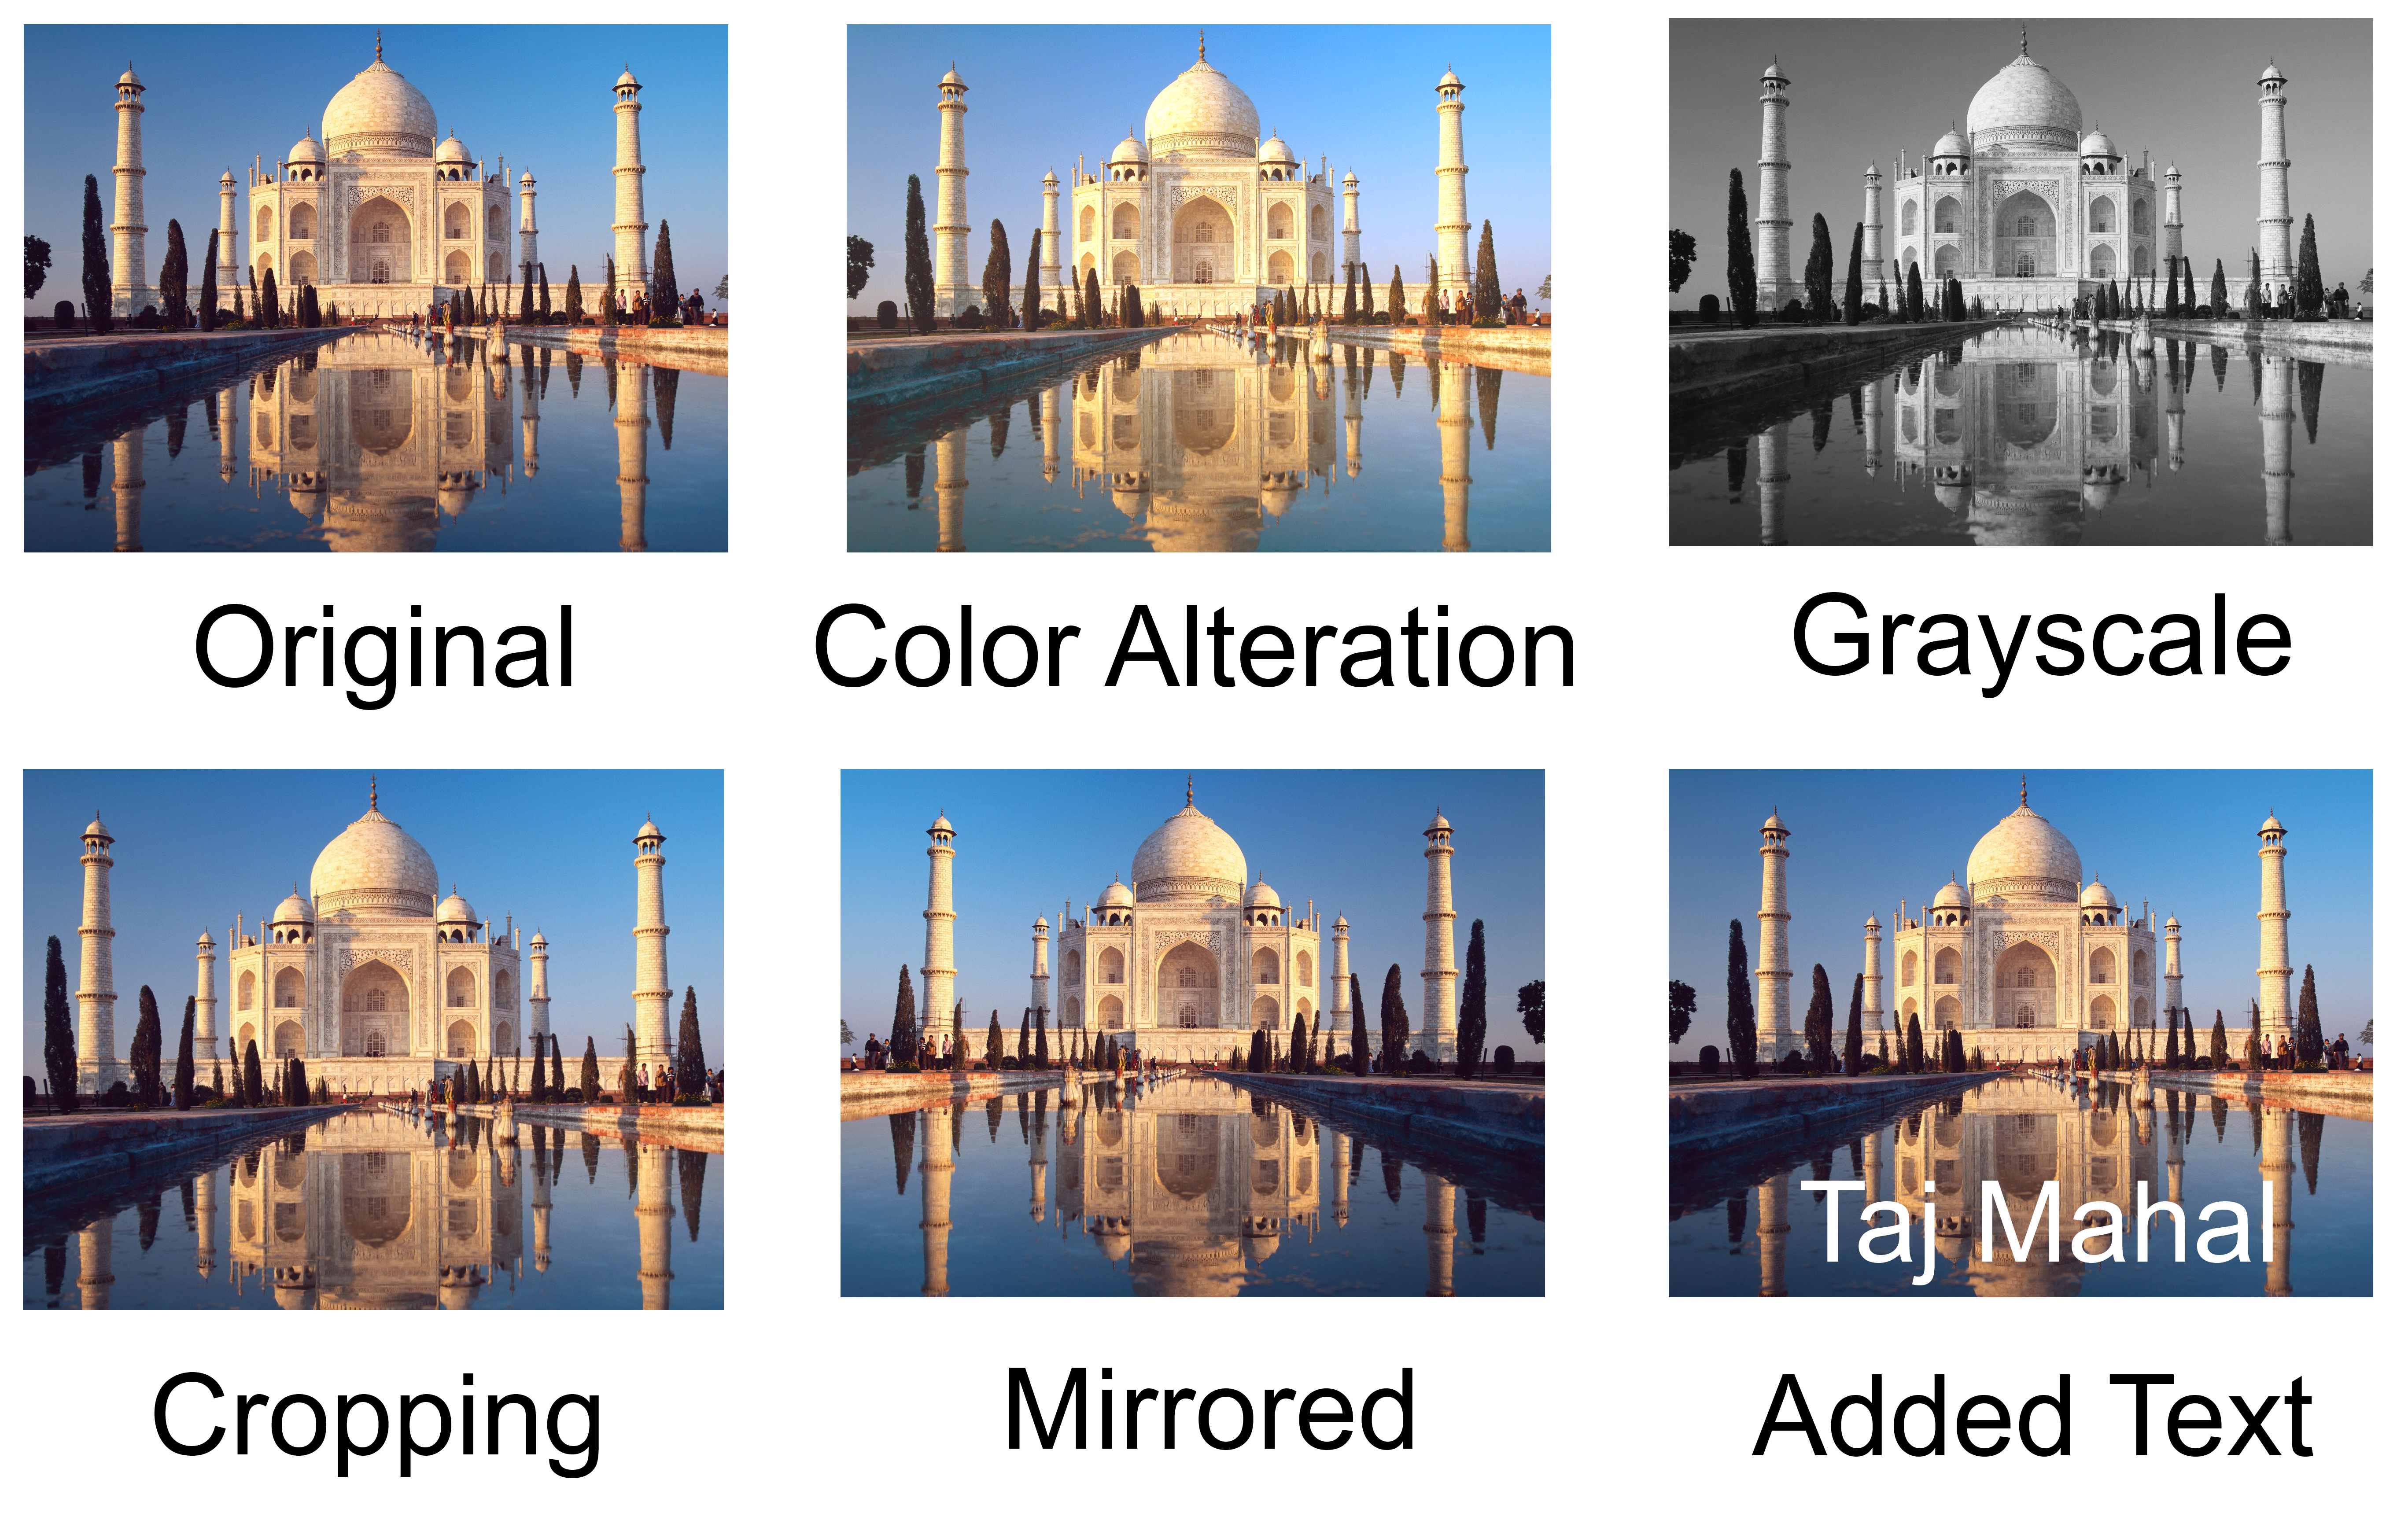
\includegraphics[width=3.5in]{imagesamples}
\caption{Possible image manipulations}
\label{imgsample}
\end{figure}

When using this thumbnail method, the authors were able to adjust automatically for differences in resolution, arbitrary amounts of cropping, caption, logo, and other manipulations, in addition to color and rotation variations, examples which can be seen in figure \ref{imgsample}. Implementing this method could benefit the research being proposed, as each of these are highly probable manipulations, and will likely each be included in the final tests performed on the implemented system.

Due to the web based nature of the proposed research, another article, written by Foo, Zobel, Sinha, and Tahaghoghi in 2007 is highly related to the proposed research. This paper discusses the topic of web search based image matching \cite{Foo:2007}, mainly the finding and determination of types of copyright infringement as most near-duplicate images are derived from one source. The goal of their research was not to derive an algorithm capable of matching images, but to locate duplicate and near-duplicate images on the web using search engines, and determine the most common methods of image alteration leading to redundancy and possibly copyright infringement. Their research will be invaluable to the proposed research as it will then be possible to target the most common methods of image alteration when creating a matching algorithm. To locate their image set to work with, they used the most popular search queries of 2005 and collected the number of images, and determined the number of unique images based on the results returned. As a note, images with non-unique URLs were not included to prevent false duplicates from the same sites. In conclusion, the authors found that the most common alterations, ordered from one to 10, one being the most common, were as follows \cite{Foo:2007}:
\begin{enumerate}
\item
\textbf{Combination:} Images with more than one alteration.
\item
\textbf{Scale:} Images that differ in size.
\item
\textbf{Crop/Zoom:} Images that are cropped from the original.
\item
\textbf{Picture in Picture:} Images that contain another image.
\item
\textbf{Contrast:} Images that have adjusted contrast.
\item
\textbf{Border/Frame:} Images that have added borders or frames.
\item
\textbf{Grayscale:} Images that have been converted to grayscale.
\item
\textbf{Recoloring:} Images with colors that have been modified.
\item
\textbf{Mirror:} Images that have been mirrored to prevent copyright infringement detection.
\item
\textbf{Rotate:} Images that have been rotated.
\end{enumerate}

The research proposed will not focus on every one of these common parameters that have been found, but will focus on a select group of these common alterations outlined in section \ref{ch:reseval}.

Finally, the most relevant information found will provide a starting codebase for the algorithm and research. An online coding tutorial provider, CatPa, outlined a method of using PHP libraries to generate real-time thumbnails and hashes of images and compare them to ones currently located on a server before uploading \cite{catpa:gdcode}. If the image is a duplicate it would be denied the privilege of being uploaded and the function would notify the user. This system is extremely limited as it provides the user with no way of adding an image to the server if it is not a duplicate and is only a false positive, and if it is unique, does not provide them with a method of accessing the already-present file.

The image comparison code developed by CatPa will be used as a base to generate a fully functional image sharing site with duplicate-reduction systems and allow for the testing of the effectiveness of such a system over traditional methods of sharing with duplicates allowed. The system created by the author \cite{catpa:gdcode} generates a $16\times 16$ thumbnail of each image on the server, and of the image being uploaded. From here, the algorithm will generate and compare black and white and color histograms, the thumbnails, and determine if it is a duplicate based on the allowable difference threshold setting which will be determined after running initial tests outlined in section \ref{ch:reseval} and analyzing the results \cite{catpa:gdcode}. The proposed research will utilize this exact method, but will provide code improvements to utilize less memory by implementing the PHP Improved libraries and also checking images for immediate similarities in resolution, exact image matching with a full MD5 image hash, and by comparison of metadata. These methods require minimal calculation, just a simple comparison of strings compared to the generation of histograms and resizing of images. After the initial string comparison approach, the code will be used to calculate the average deviation between the two images and will allow easy expansion of the system to provide a faster, more effective image matching system.

\section{Recent Results}
Recent results still being compiled and coming soon.